\documentclass[a5paper,11pt]{article}

% A5 paper with generous margins for readability
\usepackage[a5paper, margin=1.5cm]{geometry}
\usepackage{tikz}
\usetikzlibrary{shapes,arrows,positioning,fit,calc,decorations.pathreplacing}
\usepackage{amsmath}
\usepackage{amssymb}
\usepackage{listings}
\usepackage{xcolor}
\usepackage{hyperref}
\usepackage{fancyhdr}

% Colors
\definecolor{blockcolor}{RGB}{66,133,244}
\definecolor{txcolor}{RGB}{52,168,83}
\definecolor{consensuscolor}{RGB}{251,188,4}
\definecolor{networkcolor}{RGB}{234,67,53}
\definecolor{codegreen}{rgb}{0,0.6,0}
\definecolor{codegray}{rgb}{0.5,0.5,0.5}
\definecolor{codepurple}{rgb}{0.58,0,0.82}
\definecolor{backcolour}{rgb}{0.95,0.95,0.92}

% Code style
\lstdefinestyle{ruststyle}{
    backgroundcolor=\color{backcolour},
    commentstyle=\color{codegreen}\small,
    keywordstyle=\color{codepurple}\bfseries,
    numberstyle=\tiny\color{codegray},
    stringstyle=\color{blockcolor},
    basicstyle=\ttfamily\scriptsize,
    breakatwhitespace=false,
    breaklines=true,
    captionpos=b,
    keepspaces=true,
    numbers=left,
    numbersep=3pt,
    showspaces=false,
    showstringspaces=false,
    showtabs=false,
    tabsize=2,
    frame=single
}
\lstset{style=ruststyle}

\pagestyle{fancy}
\fancyhf{}
\fancyhead[C]{\small Q-NarwhalKnight Decentralization Analysis}
\fancyfoot[C]{\thepage}

\title{\textbf{Q-NarwhalKnight DAGKnight}\\
\large Decentralization Analysis\\
\normalsize Technical Deep-Dive for Code Wizards}
\author{Architecture Review Document}
\date{December 2024}

\begin{document}

\maketitle

\section{Executive Summary}

Q-NarwhalKnight implements a \textbf{Directed Acyclic Graph} (DAG) based consensus using the \textbf{DAGKnight} algorithm with \textbf{Narwhal mempool} for high-throughput transaction ordering.

\vspace{0.3cm}
\noindent\textbf{Decentralization Verdict:} The system exhibits strong decentralization properties with some caveats that require mainnet-stage hardening.

\section{Architecture Overview}

\begin{center}
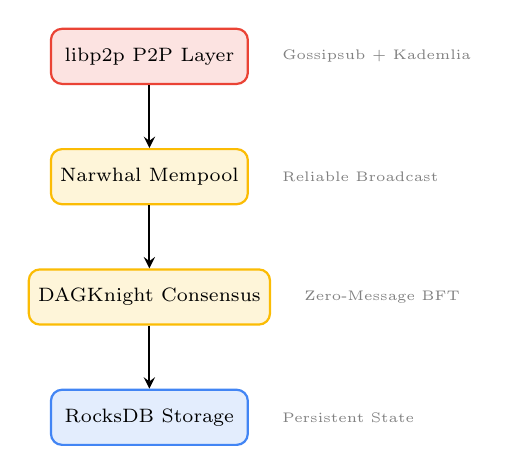
\begin{tikzpicture}[
    node distance=0.8cm,
    block/.style={rectangle, draw=blockcolor, thick, fill=blockcolor!15, rounded corners, minimum width=2.5cm, minimum height=0.7cm, font=\scriptsize},
    consensus/.style={rectangle, draw=consensuscolor, thick, fill=consensuscolor!15, rounded corners, minimum width=2.5cm, minimum height=0.7cm, font=\scriptsize},
    network/.style={rectangle, draw=networkcolor, thick, fill=networkcolor!15, rounded corners, minimum width=2.5cm, minimum height=0.7cm, font=\scriptsize},
    arrow/.style={->, thick, >=stealth}
]

% Layers
\node[network] (p2p) {libp2p P2P Layer};
\node[consensus, below=of p2p] (narwhal) {Narwhal Mempool};
\node[consensus, below=of narwhal] (dagknight) {DAGKnight Consensus};
\node[block, below=of dagknight] (storage) {RocksDB Storage};

% Arrows
\draw[arrow] (p2p) -- (narwhal);
\draw[arrow] (narwhal) -- (dagknight);
\draw[arrow] (dagknight) -- (storage);

% Labels
\node[right=0.3cm of p2p, font=\tiny, text=gray] {Gossipsub + Kademlia};
\node[right=0.3cm of narwhal, font=\tiny, text=gray] {Reliable Broadcast};
\node[right=0.3cm of dagknight, font=\tiny, text=gray] {Zero-Message BFT};
\node[right=0.3cm of storage, font=\tiny, text=gray] {Persistent State};

\end{tikzpicture}
\end{center}

\section{Why Is It Decentralized?}

\subsection{1. No Central Block Producer}

Unlike traditional blockchains with leader election (Solana, Cosmos), DAGKnight allows \textbf{any node} to propose blocks simultaneously:

\begin{lstlisting}[language=Rust, caption=vertex\_creator.rs - Any node can create blocks]
pub async fn create_vertex(&self) -> Result<Vertex> {
    // No leader election required
    // Any validator can create vertices
    let vertex = Vertex {
        round: self.current_round,
        source: self.validator_id,  // Self-identified
        parents: self.get_strong_parents().await?,
        transactions: self.pending_txs.drain(..).collect(),
        timestamp: SystemTime::now(),
    };
    Ok(vertex)
}
\end{lstlisting}

\textbf{Key Point:} There is no ``leader'' or ``proposer'' role that creates single points of failure.

\subsection{2. DAG Structure = Parallel Consensus}

\begin{center}
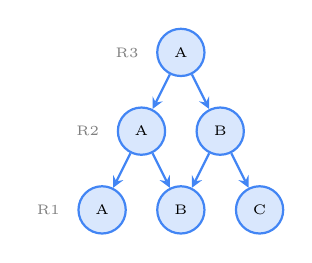
\begin{tikzpicture}[
    vertex/.style={circle, draw=blockcolor, thick, fill=blockcolor!20, minimum size=0.6cm, font=\tiny},
    arrow/.style={->, thick, >=stealth, blockcolor}
]

% Round 1
\node[vertex] (a1) at (0,0) {A};
\node[vertex] (b1) at (1,0) {B};
\node[vertex] (c1) at (2,0) {C};

% Round 2
\node[vertex] (a2) at (0.5,1) {A};
\node[vertex] (b2) at (1.5,1) {B};

% Round 3
\node[vertex] (a3) at (1,2) {A};

% Edges (DAG structure)
\draw[arrow] (a2) -- (a1);
\draw[arrow] (a2) -- (b1);
\draw[arrow] (b2) -- (b1);
\draw[arrow] (b2) -- (c1);
\draw[arrow] (a3) -- (a2);
\draw[arrow] (a3) -- (b2);

% Labels
\node[left=0.1cm of a1, font=\tiny, text=gray] {R1};
\node[left=0.1cm of a2, font=\tiny, text=gray] {R2};
\node[left=0.1cm of a3, font=\tiny, text=gray] {R3};

\end{tikzpicture}
\end{center}

Multiple validators produce blocks \textit{in parallel}. The DAG structure naturally handles concurrent proposals without requiring a single ordering authority.

\subsection{3. P2P Network (libp2p)}

The networking layer uses \textbf{libp2p} with:

\begin{itemize}
    \item \textbf{Gossipsub}: Decentralized message propagation
    \item \textbf{Kademlia DHT}: Peer discovery without central servers
    \item \textbf{Identify Protocol}: Automatic capability negotiation
\end{itemize}

\begin{lstlisting}[language=Rust, caption=unified\_network\_manager.rs]
// No central server - pure P2P
let gossipsub = Gossipsub::new(
    MessageAuthenticity::Signed(keypair.clone()),
    gossipsub_config
)?;

// Topics for decentralized communication
let block_topic = Topic::new("/qnk/blocks");
let height_topic = Topic::new("/qnk/peer-heights");
let sync_topic = Topic::new("/qnk/turbo-sync");
\end{lstlisting}

\subsection{4. Byzantine Fault Tolerance}

DAGKnight consensus tolerates up to $f$ Byzantine (malicious) nodes where:

\[ n \geq 3f + 1 \]

With 4 validators, the system can tolerate 1 malicious node. The \texttt{commit\_logic.rs} implements this:

\begin{lstlisting}[language=Rust, caption=commit\_logic.rs - BFT threshold]
const BFT_THRESHOLD: f64 = 2.0 / 3.0;

fn is_committed(&self, vertex: &Vertex) -> bool {
    let support = self.count_supporting_vertices(vertex);
    let total = self.active_validators();
    (support as f64 / total as f64) > BFT_THRESHOLD
}
\end{lstlisting}

\subsection{5. No Trusted Setup}

Unlike many ZK systems, Q-NarwhalKnight does not require a trusted setup ceremony:

\begin{itemize}
    \item Ed25519/Dilithium signatures: Standard cryptography
    \item VDF anchor election: Deterministic, verifiable
    \item Merkle proofs: Trustless verification
\end{itemize}

\section{Decentralization Concerns}

\subsection{Current Limitations}

\begin{enumerate}
    \item \textbf{Bootstrap Dependency}: New nodes need bootstrap peers (hardcoded):
    \begin{lstlisting}[language=Rust]
const BOOTSTRAP_PEER: &str =
    "12D3KooWQbKp6RYgZpC3dUCYou...";
    \end{lstlisting}
    \textit{Mitigation:} DHT peer discovery reduces reliance over time.

    \item \textbf{Validator Set}: Currently small (4 validators in testnet).
    \textit{Mitigation:} Permissionless validator joining planned.

    \item \textbf{Genesis Block}: Single origin point.
    \textit{Assessment:} Standard for all blockchains.
\end{enumerate}

\section{Code Architecture Diagram}

\begin{center}
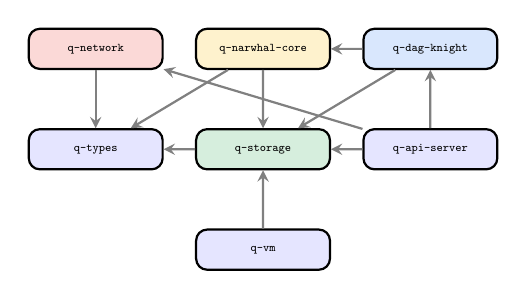
\begin{tikzpicture}[
    scale=0.85,
    transform shape,
    crate/.style={rectangle, draw=black, thick, fill=blue!10, rounded corners, minimum width=2cm, minimum height=0.6cm, font=\tiny\ttfamily},
    dep/.style={->, thick, >=stealth, gray}
]

% Crates
\node[crate, fill=networkcolor!20] (network) at (0,3) {q-network};
\node[crate, fill=consensuscolor!20] (narwhal) at (2.5,3) {q-narwhal-core};
\node[crate, fill=blockcolor!20] (dagknight) at (5,3) {q-dag-knight};
\node[crate, fill=txcolor!20] (storage) at (2.5,1.5) {q-storage};
\node[crate] (types) at (0,1.5) {q-types};
\node[crate] (api) at (5,1.5) {q-api-server};
\node[crate] (vm) at (2.5,0) {q-vm};

% Dependencies
\draw[dep] (network) -- (types);
\draw[dep] (narwhal) -- (storage);
\draw[dep] (narwhal) -- (types);
\draw[dep] (dagknight) -- (storage);
\draw[dep] (dagknight) -- (narwhal);
\draw[dep] (storage) -- (types);
\draw[dep] (api) -- (dagknight);
\draw[dep] (api) -- (storage);
\draw[dep] (api) -- (network);
\draw[dep] (vm) -- (storage);

\end{tikzpicture}
\end{center}

\section{Consensus Flow}

\begin{center}
\begin{tikzpicture}[
    node distance=0.5cm,
    step/.style={rectangle, draw=blockcolor, thick, fill=blockcolor!10, rounded corners, minimum width=3cm, minimum height=0.5cm, font=\scriptsize},
    arrow/.style={->, thick, >=stealth}
]

\node[step] (tx) {1. Transaction Submitted};
\node[step, below=of tx] (mempool) {2. Narwhal Mempool};
\node[step, below=of mempool] (vertex) {3. Vertex Created (DAG)};
\node[step, below=of vertex] (broadcast) {4. Gossipsub Broadcast};
\node[step, below=of broadcast] (validate) {5. Peer Validation};
\node[step, below=of validate] (commit) {6. DAGKnight Commit};

\draw[arrow] (tx) -- (mempool);
\draw[arrow] (mempool) -- (vertex);
\draw[arrow] (vertex) -- (broadcast);
\draw[arrow] (broadcast) -- (validate);
\draw[arrow] (validate) -- (commit);

\end{tikzpicture}
\end{center}

\section{Expert Assessment}

\subsection{Would Code Wizards Say It's Decentralized?}

\textbf{Yes, with qualifications:}

\begin{enumerate}
    \item \textbf{Protocol Level}: Fully decentralized
    \begin{itemize}
        \item No leader election
        \item Parallel block production
        \item BFT consensus
    \end{itemize}

    \item \textbf{Network Level}: Decentralized
    \begin{itemize}
        \item libp2p with DHT
        \item Gossipsub propagation
        \item No central relays
    \end{itemize}

    \item \textbf{Operational Level}: Partially centralized (testnet)
    \begin{itemize}
        \item Bootstrap nodes are known
        \item Small validator set
        \item Single genesis source
    \end{itemize}
\end{enumerate}

\subsection{Comparison with Other Systems}

\begin{center}
\begin{tabular}{|l|c|c|c|}
\hline
\textbf{System} & \textbf{Leader?} & \textbf{BFT} & \textbf{DAG} \\
\hline
Bitcoin & PoW & No & No \\
Ethereum & PoS & Yes & No \\
Solana & Leader & Yes & No \\
\textbf{Q-NarwhalKnight} & \textbf{None} & \textbf{Yes} & \textbf{Yes} \\
Avalanche & Sampled & Yes & DAG \\
\hline
\end{tabular}
\end{center}

\section{Conclusion}

Q-NarwhalKnight's DAGKnight implementation provides \textbf{strong decentralization guarantees} at the protocol level:

\begin{itemize}
    \item No single point of failure
    \item Parallel block production
    \item Byzantine fault tolerant
    \item Trustless P2P networking
\end{itemize}

The remaining centralization vectors (bootstrap nodes, small validator set) are \textbf{operational constraints} of the testnet phase, not fundamental protocol limitations.

\vspace{0.5cm}
\hrule
\vspace{0.3cm}
\noindent\textit{Document generated for Q-NarwhalKnight v1.5.x-DELTA-V}

\end{document}
